\documentclass[12pt]{article}
\usepackage[utf8]{inputenc}

\usepackage{lmodern}

\usepackage{enumitem}
\usepackage[margin=2cm]{geometry}

\usepackage{amsmath, amsfonts, amssymb}
\usepackage{graphicx}
%\usepackage{subfigure}
\usepackage{tikz}
\usepackage{pgfplots}
\usepackage{multicol}

\usepackage{comment}
\usepackage{url}
\usepackage{calc}
\usepackage{subcaption}
\usepackage[indent=0pt]{parskip}
\usepackage{animate}

\usepackage{array}
\usepackage{blkarray,booktabs, bigstrut}
\usepackage{bigints}

\pgfplotsset{compat=1.16}

% MATH commands
\newcommand{\ga}{\left\langle}
\newcommand{\da}{\right\rangle}
\newcommand{\oa}{\left\lbrace}
\newcommand{\fa}{\right\rbrace}
\newcommand{\oc}{\left[}
\newcommand{\fc}{\right]}
\newcommand{\op}{\left(}
\newcommand{\fp}{\right)}

\newcommand{\bi}{\mathbf{i}}
\newcommand{\bj}{\mathbf{j}}
\newcommand{\bk}{\mathbf{k}}
\newcommand{\bF}{\mathbf{F}}

\newcommand{\mR}{\mathbb{R}}

\newcommand{\ra}{\rightarrow}
\newcommand{\Ra}{\Rightarrow}

\newcommand{\sech}{\mathrm{sech}\,}
\newcommand{\csch}{\mathrm{csch}\,}
\newcommand{\curl}{\mathrm{curl}\,}
\newcommand{\dive}{\mathrm{div}\,}

\newcommand{\ve}{\varepsilon}
\newcommand{\spc}{\vspace*{0.5cm}}

\DeclareMathOperator{\Ran}{Ran}
\DeclareMathOperator{\Dom}{Dom}

\newcommand{\exo}[1]{\noindent\textcolor{red}{\fbox{\textbf{Problem {#1}}}\hrulefill}\\\\ }
\newcommand{\qu}[4]{\noindent\textcolor{#4}{\fbox{\textbf{Section {#1} | Problem {#2}}} \hrulefill{{\fbox{\textbf{{#3} Points}}}}\\}}

\newcommand{\semester}{Fall 2023}

\newcommand{\CVup}{%

\begin{tikzpicture}
\draw[black, <->, >=latex] (-0.33, 0.5) .. controls (-0.125, 0) and (0.125, 0) .. (0.33, 0.5);
\end{tikzpicture}}

\newcommand{\CVupInc}{%
\begin{tikzpicture}
\draw[black, ->, >=latex] (0,0) .. controls (0.2, 0) and (0.4, 0.2) .. (0.5, 0.5);
\end{tikzpicture}}

\newcommand{\CVupDec}{%
\begin{tikzpicture}[rotate=270]
\draw[black, ->, >=latex] (0,0) .. controls (0.2, 0) and (0.4, 0.2) .. (0.5, 0.5);
\end{tikzpicture}}

\newcommand{\CVdown}{%
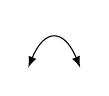
\begin{tikzpicture}
\draw[black, <->, >=latex] (-0.33, -0.5) .. controls (-0.125, 0) and (0.125, 0) .. (0.33, -0.5);
\end{tikzpicture}}

\newcommand{\CVdownInc}{%
\begin{tikzpicture}
\draw[black, ->, >=latex] (-0.5, -0.5) .. controls (-0.5, -0.3) and (-0.5, -0.1) .. (0,0);
\end{tikzpicture}}

\newcommand{\CVdownDec}{%
\begin{tikzpicture}[rotate=-90]
\draw[black, ->, >=latex] (-0.5, -0.5) .. controls (-0.5, -0.3) and (-0.5, -0.1) .. (0,0);
\end{tikzpicture}}

\begin{document}
	\noindent \hrulefill \\
	MATH-244 \semester \hfill Practice Problems Solutions\\
	Section 16.3 \hfill Pierre-Olivier Paris{\'e} \\\vspace*{-1cm}
	
	\noindent\hrulefill
	
	\spc	

	\exo{4}
	\\
	We have $P (x, y) = y^2 - 2x$ and $Q(x, y) = 2xy$. Then, we see that
		\begin{align*}
		P_y = 2y \quad \text{ and } \quad Q_x = 2y .
		\end{align*}
	So $P_y = Q_x$ and the vector field $\vec{F}$ is conservative.
	
	So, there is a function $f$ such that $\vec{F} = \vec{\nabla} f = f_x \vec{i} + f_y \vec{j}$. We must have
		\begin{align*}
		f_x = y^2 - 2x \quad \text{ and } \quad f_y = 2xy .
		\end{align*}
	Integrating with respect to $x$, we find out that $f(x, y) = y^2x - x^2 + g(y)$. Then, differentiating with respect to $y$, we find $f_y (x, y) = 2xy + g'(y) = 2xy$ and so $g'(y) = 0$. This implies that $g(y) = C$ for a constant $C$. Thus,
		\begin{align*}
		f(x, y) = xy^2 - x^2 + C. 
		\end{align*}
		
	\spc
	
	\exo{20}
	\\
	If $\vec{r}(t) = (x(t) , y(t))$, with $a \leq t \leq b$ is a parametrization of the path $C$, then the line integral can be expressed as
		\begin{align*}
		\int_a^b \vec{F} (\vec{r}(t)) \cdot \vec{r}\,' (t) \, dt .
		\end{align*}
	where $\vec{F} (x, y) = \left\langle \sin y , x \cos y - \sin y \right\rangle$.
	
	Now, it is sufficient to show that $\vec{F}$ is conservative. We have $P(x, y) = \sin y$ and $Q (x, y) = x \cos y - \sin y$, so
		\begin{align*}
		P_y = \cos y \quad \text{ and } \quad Q_x = \cos y .
		\end{align*}
	We see that $P_y = Q_x$ and so $\vec{F}$ is conservative. 
	
	We now need to find a potential function $f$. By repeating the procedure from the previous exercise, we obtain
		\begin{align*}
		f(x, y) = x \sin y + \cos (y) .
		\end{align*}
	So by the fundamental Theorem for line integrals, we get
		\begin{align*}
		\int_C \sin y dx + (x \cos y - \sin y) \, dy = f(1, \pi ) - f(2, 0) = -1 + 1 = 0 .
		\end{align*}


\end{document}